\section{L'Equazione Logistica}

L'equazione logistica è un modello matematico adatto a descrivere una vasta gamma di fenomeni, inoltre è estremamente semplice per cui risulta molto utile per introdurre varie considerazioni di base che possiamo fare nello studio di un fenomeno.

\subsection{Il modello}

Consideriamo un popolazione di cui vogliamo studiare la dinamica: cerchiamo quindi di modellizzarla molto semplicemente, per farlo possiamo utilizzare un \textbf{automa cellulare}.\\

Per prima cosa possiamo discretizzare lo spazio dove vive la popolazione e il tempo con cui evolve. Per farlo costruiamo una tabella in cui ogni cella può essere occupata da un individuo e la facciamo evolvere applicando delle regole stabilite ogni $\Delta t$.
\begin{center}
	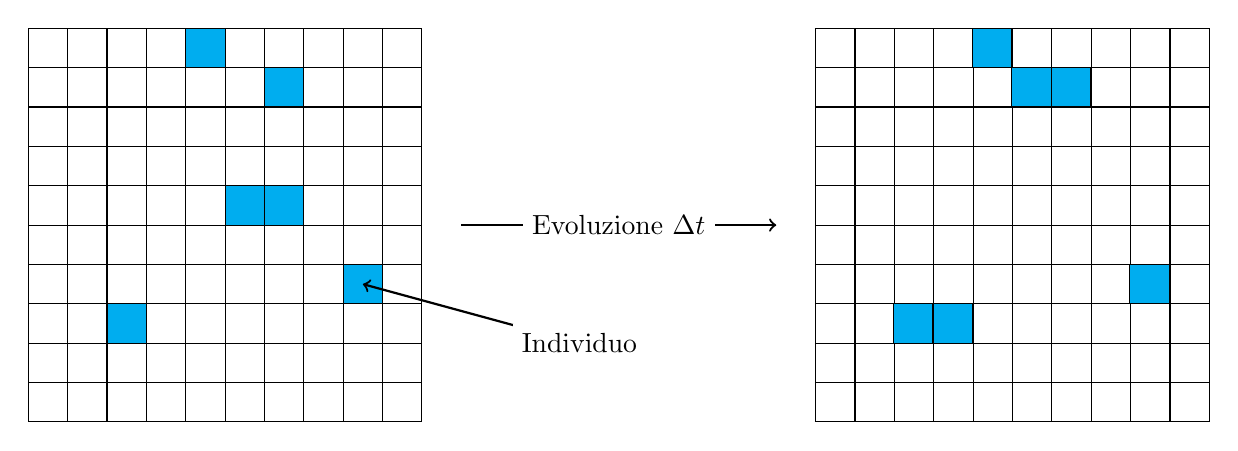
\begin{tikzpicture}
		\draw[step=0.5cm] (0,0) grid (5,5);
		\draw[step=0.5cm] (9.99,0) grid (15,5);
		
		\filldraw[fill=cyan] (1,1) rectangle (1.5,1.5);
		\filldraw[fill=cyan] (3,4) rectangle (3.5,4.5);
		\filldraw[fill=cyan] (4,1.5) rectangle (4.5,2);
		\filldraw[fill=cyan] (2,4.5) rectangle (2.5,5);
		\filldraw[fill=cyan] (2.5,2.5) rectangle (3,3);
		\filldraw[fill=cyan] (3,2.5) rectangle (3.5,3);
		
		\draw[->,thick] (5.5,2.5) -- (9.5,2.5);
		\node[fill=white] at (7.5,2.5) {Evoluzione $\Delta t$};
		
		\filldraw[fill=cyan] (10.99,1) rectangle (11.49,1.5);
		\filldraw[fill=cyan] (12.99,4) rectangle (13.49,4.5);
		\filldraw[fill=cyan] (13.99,1.5) rectangle (14.49,2);
		\filldraw[fill=cyan] (11.99,4.5) rectangle (12.49,5);
		\filldraw[fill=cyan] (12.49,4) rectangle (12.99,4.5);
		\filldraw[fill=cyan] (11.49,1) rectangle (11.99,1.5);
		
		\draw[<-,thick] (4.25,1.75) -- (7,1);
		\node[fill=white] at (7,1) {Individuo};
	\end{tikzpicture}
\end{center}
Le regole che descrivono le dinamiche caratteristiche del sistema sono in questo caso di \textbf{riproduzione-competizione}:

\begin{itemize}
	\item \textbf{Riproduzione}: un individuo si può riprodurre ogni $\Delta t$ se nelle celle adiacenti non ci sono individui con cui competere per il cibo.
	\item \textbf{Competizione}: se un individuo è circondato da troppi contendenti allora muore.
\end{itemize}

Questa tipologia di modello può quindi essere simulata al computer, per poterne facilitare lo studio. Infatti la discretizazione da un lato diminuisce l'aderenza del modello con la realtà ma lo rende più adatto alla simulazione.\\

A questo punto cerchiamo di tradurre il modello in termini matematici. Se chiamiamo $n(t)$ la popolazione al tempo $t$ è immediato dedurre che:

\begin{itemize}
	\item $\Delta n_{Riproduzione} \ \propto \ n(t)$
	\item $\Delta n_{Competizione} \ \propto \ -n^2(t)$
\end{itemize}

Infatti ogni individuo può potenzialmente riprodursi, per cui gli individui nati dopo un $\Delta t$ è maggiore tanto quanto lo sono gli individui totali. Un individuo può invece competere con $n-1$ individui, ossia tutti gli altri, ma poichè gli individui totali sono $n$ allora in totale quelli morti dopo un $\Delta t$ sono proporzionali alle possibili coppie di interazione $n(n-1)\sim n^2$, per cui possiamo scrivere:

\begin{equation}
	n(t+\Delta t)=n(t)+(an(t)-bn^2(t))\Delta t
	\label{logDisc}
\end{equation}

Se consideriamo $\Delta t$ piccolo possiamo passare al continuo ottenendo dalla (\ref{logDisc}) l'\textbf{equazione logistica}:

\begin{equation}
\dot{n}(t)=an(t)(1-\frac{b}{a}n(t)) \label{logequation}
\end{equation}

\subsection{Studio del modello}

Dopo aver ricavato l'equazione che regola il modello possiamo passare ad uno studio matematico procedendo per punti:

\begin{enumerate}
	\item \textbf{In quale spazio mi muovo?} In questo caso $n(t)\in\mathbb{R}^+$
	\item \textbf{Quali sono i punti di equilibrio?} Equilibrio $\Longleftrightarrow$ $\dot{n}(t)=0$ \\ In questo caso abbiamo che $n_{eq}= 0 $ oppure $ n_{eq}= \frac{a}{b}$.
	\item \textbf{Gli equilibri sono stabili o instabili?} \\ Per studiare gli equilibri perturbiamo la soluzione all'equilibrio e studiamo cosa accade alla soluzione:
	\begin{equation}
		\delta n=n(t)-n_{eq} \ \Rightarrow \ \delta \dot{n}=\dot{n}(t)=an(t)(1-\frac{b}{a}n(t))
		\label{logPerturb}
	\end{equation}
     Sostituendo $\delta n$ al posto di $n(t)$ in tutta la (\ref{logPerturb}) troviamo un'equazione differenziale che possiamo linearizzare per studiarla nell'intorno dell'equilibrio.
     \begin{equation}
     	\delta \dot{n}=a(\delta n- n_{eq})-b(\delta n- n_{eq})^2\sim (a-2bn_{eq})\delta n+an_{eq}-bn^2_{eq}
     \end{equation}
 Risulta quindi immediato che se $n_{eq}=0$ allora $\delta n(t)=\delta n_0 e^{at}$, ossia che è un punto di equilibrio instabile, poichè le perturbazioni si allontanano dall'equilibrio. Se $n_{eq}=\frac{a}{b}$ allora la soluzione sarà  $\delta n(t)=\delta n_0 e^{-at}$, per cui la perturbazione tende a convergere sul punto di equilibrio che è quindi stabile.
\end{enumerate}

\subsection{Leggi di scala}

Un'ultima osservazione che possiamo fare sulla (\ref{logequation}) riguarda come riscalano la popolazione e il tempo e come cambia l'equazione. Poniamo quindi il seguente \textbf{riscalamento}:

\begin{equation}
	t\longrightarrow\mu t \qquad n\longrightarrow\lambda n
\end{equation}
applicandolo alla (\ref{logequation}) otteniamo :
\begin{equation}
	\dot{n}(t)=an(t)(1-\frac{b}{a}n(t))\longrightarrow\dot{n}(t)=\mu an(t)-b\mu \lambda n^2(t))
\end{equation}
che osserviamo ridursi ad un'equazione senza parametri se $\mu=a^{-1}$ e $\lambda=\frac{a}{b}$. Questo ci suggerisce che i parametri $a$ e $b$ non sono intrinsecamente importanti per lo studio del modello e che quindi sono solamente le condizioni iniziali a influenzare la soluzione. 
\subsection{La soluzione analitica}
Per terminare ricaviamo la soluzione analitica dell'equazione logistica, per farlo integriamo per parti l'equazione priva di coefficienti, che come abbiamo mostrato con gli opportuni riscalamenti possono essere reintrodotti:
\begin{center}
	
\begin{equation*}
	\begin{gathered}
		\dot{x}=x(1-x)\qquad \Rightarrow \qquad \int_{x_0}^x \frac{ds}{s(1-s)}=\int_0^tdu\\\\
		\int_{x_0}^x \left[ \frac{1-s}{s(1-s)}+\frac{s}{s(1-s)} \right]ds=\int_{x_0}^x \left[ \frac{1}{s}+\frac{1}{(1-s)} \right]ds=t\\\\
		\log\frac{x}{x_0}-\log\frac{1-x}{1-x_0}=\log\frac{x}{1-x} - \log\frac{x_0}{1-x_0}=t\\\\	
		\frac{x}{1-x}=\frac{x_0}{1-x_0}e^t
	\end{gathered}
\end{equation*}

\end{center}\paragraph{Funzione Logistica}
Con un po' di algebra e raccogliendo tutte le costanti in una unica si ottiene la \textbf{funzione logistica}:

\begin{center}
	\begin{equation}
	x(t)=\frac{ce^t}{1+ce^t}
	\label{logfunction}
\end{equation}


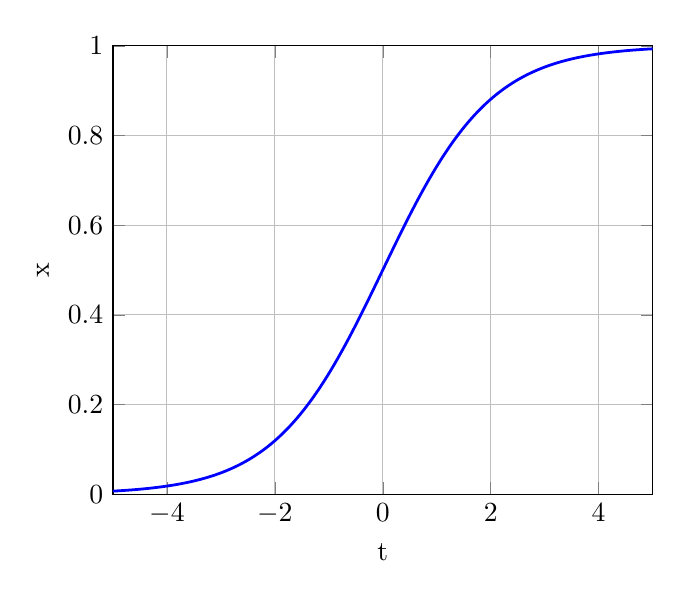
\begin{tikzpicture}
	\begin{axis}[xmin = -5, xmax = 5,
		ymin = 0, ymax = 1,
		grid, xlabel = t, ylabel = x,
		samples=500
		]
		\addplot[% opzioni di disegno
		color=blue, line width=1pt
		] {
			exp(x)/(1+exp(x)) % espressione matematica
		};
	\end{axis}
    \label{graph}
\end{tikzpicture}
\end{center}
Osserviamo che la funzione trovata ha effettivamente il comportamento atteso: cresce esponenzialmente da $x=0$ (eq. instabile) per poi decrescere esponenzialmente verso il valore massimo $x=1$ (eq. stabile). 